\section{问题四：波动电价下的两层调度}
\subsection{给定电价G与历史预测H}
主口径G直接采用附件4的当日及次日电价替换两日规划中的固定价格，负荷和光伏信息范围保持不变。
年末没有下一年度价格时，对第二日价格沿用最后可得日的曲线；第二日仅作为窗口延伸，不进入本年度报送费用。
该模型评价在题目给定价格条件下能够达到的调度效果，不能将其解释为价格未知时的可实现收益。

为考察电价信息受限情况，扩展H采用三源预测
\begin{equation}
\widehat p_{d,t}=v_{d,1}p_{d-1,t}+v_{d,2}p_{d-7,t}+v_{d,3}\bar p_t,
\qquad v_{d,i}\geq0,\ \sum_i v_{d,i}=1.
\label{eq:price}
\end{equation}
候选权重按此前7天费用选择，再进行$v_d=0.1v_d^\ast+0.9v_{d-1}$平滑。
预测次日时，尚未实现的当日价格用最近已观测曲线替代。
H只改变优化时的价格输入，最终计划、偏差和紧急费用仍按实际交易价格结算。

\subsection{无调整层与调整层结果}
问题四分别沿用问题二与问题三的预测、SOC与执行结构，仅替换电价。
表\ref{tab:q4}给出334天结果；G两层费用分别为1459.8、1410.3万元，H分别为1465.9、1418.4万元。
\begin{table}[htbp]\centering
\caption{波动电价下的正式结果与历史价格扩展}\label{tab:q4}
\begin{tabular}{lrr}
\toprule
指标 & 无日内调整层 & 有日内调整层\\\midrule
G总费用/万元 & 1459.8 & 1410.3\\
G紧急购电费/万元 & 92.8 & 40.5\\
G紧急购电量/kWh & 155951.8 & 77378.0\\
H总费用/万元 & 1465.9 & 1418.4\\
H相对G费用增幅 & 0.42\% & 0.57\%\\
\bottomrule
\end{tabular}
\end{table}
有调整层的费用由买入、偏差与紧急费用构成，见图\ref{fig:q4}。
日内调整降低了短缺量及紧急费用；不能将与固定价问题的费用差直接解释成策略改进或退化，因为结算价格环境已经变化。
\begin{figure}[htbp]\centering
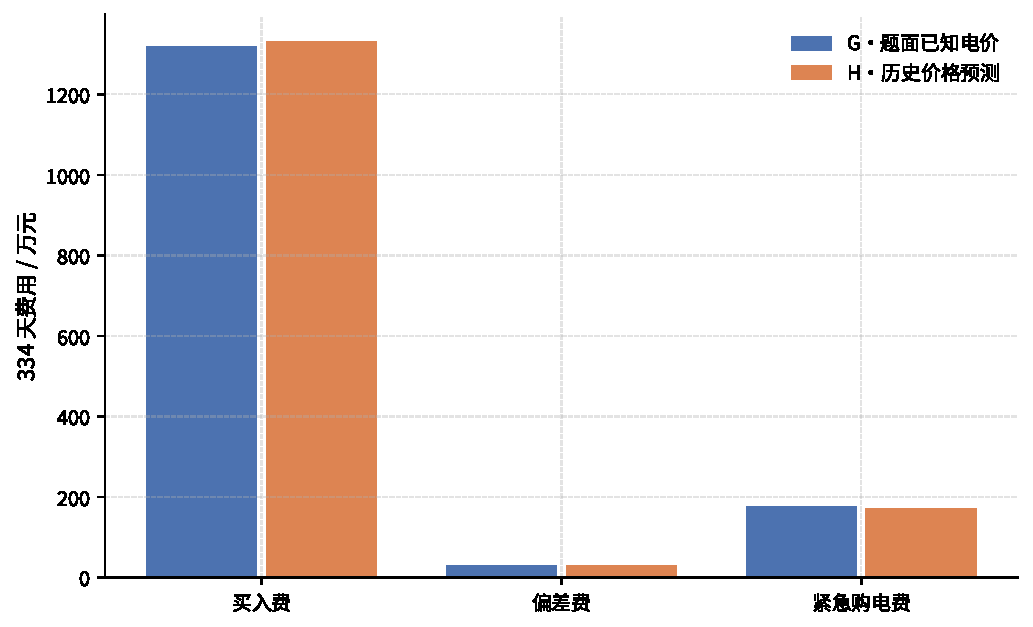
\includegraphics[width=.83\textwidth]{../../figures/Q4_调整层策略对比.pdf}
\caption{波动电价调整层在G、H两种信息条件下的费用分解}\label{fig:q4}
\end{figure}
以$I_p=(C_H-C_G)/C_G$度量条件电价信息价值，得到0.42\%和0.57\%。
该结果说明在这组数据及当前预测策略下，价格预测误差的额外成本较小；它不能推广为所有电价机制下的信息价值都很低。
G仍需面对未知的负荷与光伏，因此也不是所有不确定性消失后的理论最优下界。

\subsection{物理可行性与结果校验}
G无调整层和调整层的功率平衡最大残差分别为$4.547\times10^{-13}$与$3.411\times10^{-13}$ kWh，
SOC递推最大残差均为$1.137\times10^{-13}$ kWh；储电量落在1200至10800 kWh，同槽同时充放次数为0。
调整层正式方案不使用场景池。完整计划、最终调整、分段充放电与紧急购电事件分别写入题目指定的两份结果表。
\questionconclusion{波动价格条件下，无调整层费用1459.8万元，有调整层1410.3万元；历史电价预测扩展的额外费用分别为0.42\%与0.57\%。}
